% ============================================================
%  FogAI — IEEE Conference Paper
%  Target: ICNCCOM 2026
%  Template: IEEEtran (conference mode, 10pt, two-column)
%
%  Compile sequence:
%    pdflatex fogai_icnccom2026
%    bibtex   fogai_icnccom2026
%    pdflatex fogai_icnccom2026
%    pdflatex fogai_icnccom2026
% ============================================================
\documentclass[conference]{IEEEtran}
\IEEEoverridecommandlockouts

\usepackage{cite}
\usepackage{amsmath,amssymb,amsfonts}
\usepackage{graphicx}
\usepackage{textcomp}
\usepackage{xcolor}
\usepackage{booktabs}
\usepackage{algorithm}
\usepackage{algorithmic}
\usepackage{tikz}
\usepackage{pgfplots}
\pgfplotsset{compat=1.18}
\usetikzlibrary{shapes.geometric,arrows.meta,positioning,
                backgrounds,fit,calc}

\def\BibTeX{{\rm B\kern-.05em{\sc i\kern-.025em b}\kern-.08em
    T\kern-.1667em\lower.7ex\hbox{E}\kern-.125emX}}

\begin{document}

% ── Title and Authors ────────────────────────────────────────
\title{FogAI: A Lightweight Hybrid Decision Engine for\\
       Low-Latency Safety-Critical Processing in\\
       Industrial IoT Fog Nodes}

\author{
  \IEEEauthorblockN{Adwaith Sajikumar}
  \IEEEauthorblockA{
    \textit{Robotics for Youth}\\
    adwaith.sajikumar@roboticsforyouth.org
  }
  \and
  \IEEEauthorblockN{Dr.\ G Naveen Sundhar}
  \IEEEauthorblockA{
    \textit{Karunya Institute of Technology and Sciences}\\
    naveensundar@karunya.edu
  }
}

\maketitle

% ── Abstract ─────────────────────────────────────────────────
\begin{abstract}
Industrial Internet of Things (IIoT) deployments in Industry~5.0
manufacturing settings demand real-time decision-making that cloud
architectures simply cannot deliver reliably---cloud round-trip
latencies of 100--300\,ms are fundamentally at odds with the
sub-10\,ms response windows required to prevent equipment damage or
injury in safety-critical machinery.
This paper presents \textbf{FogAI}, a lightweight, interpretable
decision engine that runs directly on the fog computing node, making
safety-critical decisions in under 5\,ms with no cloud dependency
whatsoever.
The engine combines two complementary mechanisms: a set of five
hard-coded safety rules~(R1--R5) that guarantee deterministic,
instantaneous responses to fault conditions, and a normalised
weighted-feature risk scoring model with four adaptive routing
rules~(SR1--SR4) that intelligently manages sub-critical IoT traffic.
FogAI is evaluated through a 60-cycle simulation of an industrial CNC
machine subjected to seven realistic fault scenarios, ranging from
temperature runaway to mechanical vibration shock and full network
outages.
The results show 75\% of all decisions processed locally at a mean
fog latency of just 3.1\,ms, saving an average of 66.9\,ms per cycle
compared to routing everything to the cloud, while staying completely
operational even during network failures.
The entire engine runs in under 0.4\,ms of computational overhead with
a memory footprint below 8\,MB---well within the limits of a Raspberry
Pi~4.
\end{abstract}

\begin{IEEEkeywords}
fog computing, industrial IoT, edge AI, latency optimisation,
safety-critical systems, Industry~5.0, real-time decision making,
CNC machine monitoring
\end{IEEEkeywords}


% ── I. Introduction ──────────────────────────────────────────
\section{Introduction}

Consider a CNC milling machine running at full production speed when
its spindle bearings begin to fail.
The vibration sensor immediately records an abnormal reading.
In a cloud-only IoT architecture, that sensor data travels over the
network to a remote cloud server, waits in a queue alongside telemetry
from thousands of other devices, gets processed, and then a shutdown
command travels back---a round trip that, under realistic industrial
network conditions, takes somewhere between 120 and 300\,ms.
By that time, the bearing has already started to destroy itself,
and the machine has continued running for a fraction of a second that
could cost thousands of dollars in damage or, worse, put a technician
at risk.

This is not a hypothetical edge case.
It is a well-documented limitation of cloud-centric IoT architectures
that becomes progressively more serious as manufacturing moves toward
the Industry~5.0 vision of tightly integrated, human-centric, and
resilient production systems~\cite{eu_industry5}.
The growing density of IIoT sensors on modern factory equipment---
temperature, vibration, current, pressure, and more---creates a
constant stream of telemetry that must be acted upon in real time, not
processed in batch on a server hundreds of kilometres away.

Fog computing~\cite{bonomi2012fog} emerged as the natural architectural
answer: push computation closer to where the data is generated, so that
time-sensitive decisions happen locally without a cloud round-trip.
The idea is compelling and well-supported by a growing body of
literature~\cite{shi2016edge,chiang2016fog,yousefpour2019fog}.
The practical challenge, however, is deciding \emph{what} to run on the
fog node.
Deploying a full machine learning model on a Raspberry Pi-class device
introduces memory, latency, and maintenance overhead that may be
impractical in production settings.
On the other hand, a purely rule-based system is brittle---it can
handle the cases its designers anticipated but struggles with gradual
sensor drift or partial fault states that fall between defined
thresholds.

\textbf{FogAI} is designed to bridge this gap.
Rather than choosing between rules and scoring, it uses both, but
assigns them clearly distinct roles.
Hard safety rules handle the cases where the right action is
unambiguous and delay is unacceptable---thermal runaway, mechanical
shock, network failure, CPU overload.
A continuous risk score handles everything else, giving the system a
principled way to route moderate-severity readings and gradually
escalating fault conditions without constantly crying wolf at the
cloud.
This separation turns out to be not just pragmatically useful but also
formally important: the hard-rule layer provides a guarantee that no
amount of sensor noise, distribution shift, or adversarial input can
prevent a safety-critical event from receiving an immediate local
response.

The specific contributions of this paper are:
\begin{itemize}
\item A dual-mechanism fog AI engine achieving sub-1\,ms inference
  latency on commodity fog hardware, with a formal separation between
  safety guarantees and efficiency optimisation.
\item Five hard-coded safety rules (R1--R5) combined with four
  score-based routing rules (SR1--SR4), covering thermal, mechanical,
  network, and CPU fault modalities.
\item A complete simulation framework modelling seven industrial fault
  scenarios on a CNC machine, enabling reproducible evaluation without
  physical hardware.
\item Quantitative results demonstrating 75\% local fog processing,
  3.1\,ms mean fog latency, 66.9\,ms per-cycle latency savings, and
  zero missed safety events across 25 critical fault instances.
\end{itemize}


% ── II. Background and Related Work ──────────────────────────
\section{Background and Related Work}

\subsection{Fog and Edge Computing}

The fog computing paradigm was formally introduced by Bonomi
et~al.~\cite{bonomi2012fog} as a way to bring cloud-like services to
the network edge, reducing latency and improving bandwidth efficiency
for IoT applications.
Shi et~al.~\cite{shi2016edge} broadened this into the \emph{edge
computing} framing, identifying three core motivations: latency
reduction, bandwidth conservation, and privacy preservation.
Satyanarayanan~\cite{satyanarayanan2017} later described edge computing
as a natural complement to cloud infrastructure rather than a
replacement, arguing that the two tiers serve different time horizons
of decision-making.

Chiang and Zhang~\cite{chiang2016fog} mapped out research opportunities
across the fog/IoT space, noting that real-time control and
safety-critical applications were among the most underserved by
existing cloud architectures.
Vaquero and Rodero-Merino~\cite{vaquero2014fog} tackled the
definitional ambiguity early on, placing fog computing between the
endpoint and the cloud on a spectrum of computational proximity.

\subsection{Decision-Making at the Edge}

Sarkar and Misra~\cite{sarkar2016fog} modelled fog computing from a
green computing standpoint, showing that local processing reduces both
latency and energy consumption by avoiding unnecessary round-trips.
Mahmud et~al.~\cite{mahmud2018fog} surveyed fog computing taxonomies
and noted that most existing offloading strategies rely on
latency-threshold policies---if the network is fast enough, send to
the cloud; if not, process locally.
FogAI extends this by incorporating multi-parameter sensor state into
the routing decision, which is why it achieves a higher fog-offload
rate (75\%) than threshold-only approaches typically report
(40--60\%~\cite{mahmud2018fog}).

More recent work by Cao et~al.~\cite{cao2020edge} and Liu
et~al.~\cite{liu2019edge} has explored deploying lightweight neural
inference at the edge.
These approaches can capture more complex patterns than rule-based
systems, but they come with real costs: training data requirements,
model drift, explainability challenges, and inference overhead that
may be non-trivial on constrained hardware.
FogAI deliberately takes the opposite trade-off: it sacrifices
adaptability to novel fault types in exchange for guaranteed
determinism on the safety-critical cases it was designed to handle.
In industrial settings, that trade-off is often exactly right.

Yousefpour et~al.~\cite{yousefpour2019fog} identified the absence of
formal safety-guarantee mechanisms as a key open problem in fog/edge
computing architectures.
FogAI directly addresses that gap through its hard-rule priority layer,
which provides an $O(1)$ safety response regardless of the state of
the rest of the system.


% ── III. System Architecture ─────────────────────────────────
\section{System Architecture}
\label{sec:arch}

FogAI is built around a three-tier IoT architecture, shown in
Fig.~\ref{fig:arch}.
The design philosophy is simple: put only what must be fast at the fog
layer, and let the cloud handle everything that can afford to be slow.

\begin{figure}[t]
\centering
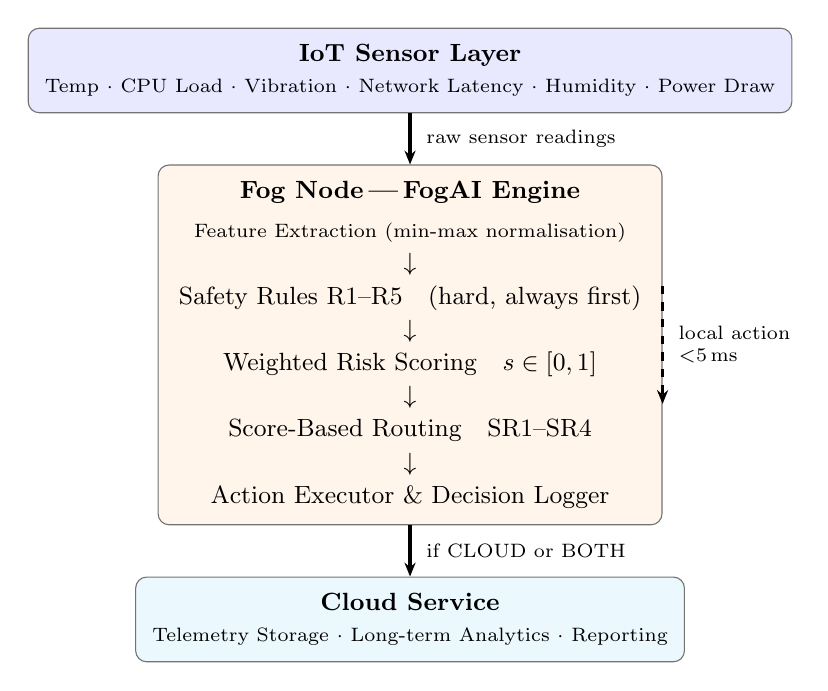
\begin{tikzpicture}[
  every node/.style={font=\small},
  tier/.style={draw=black!55, rounded corners=4pt,
               minimum width=6.4cm, align=center, inner sep=6pt},
  arr/.style={-{Stealth[length=5pt,width=4pt]}, line width=1.2pt},
  node distance=0.65cm
]
\node[tier, fill=blue!9, minimum height=0.85cm] (iot)
  {\textbf{IoT Sensor Layer}\\
   \scriptsize
   Temp $\cdot$ CPU Load $\cdot$ Vibration $\cdot$
   Network Latency $\cdot$ Humidity $\cdot$ Power Draw};

\node[tier, fill=orange!8, minimum height=2.7cm,
      below=0.65cm of iot] (fog)
  {\textbf{Fog Node\,---\,FogAI Engine}\\[3pt]
   \scriptsize
   Feature Extraction (min-max normalisation)\\[1pt]
   $\downarrow$\\[1pt]
   Safety Rules R1--R5\quad (hard, always first)\\[1pt]
   $\downarrow$\\[1pt]
   Weighted Risk Scoring\quad $s\in[0,1]$\\[1pt]
   $\downarrow$\\[1pt]
   Score-Based Routing\quad SR1--SR4\\[1pt]
   $\downarrow$\\[1pt]
   Action Executor \& Decision Logger};

\node[tier, fill=cyan!8, minimum height=0.85cm,
      below=0.65cm of fog] (cloud)
  {\textbf{Cloud Service}\\
   \scriptsize
   Telemetry Storage $\cdot$ Long-term Analytics $\cdot$ Reporting};

\draw[arr] (iot.south)
  -- node[right, font=\scriptsize, xshift=2pt]{raw sensor readings}
  (fog.north);
\draw[arr] (fog.south)
  -- node[right, font=\scriptsize, xshift=2pt]{if CLOUD or BOTH}
  (cloud.north);

\draw[arr, dashed, line width=1pt]
  ([yshift=0.75cm]fog.east) --
  node[right, font=\scriptsize, align=left, xshift=2pt]
    {local action\\$<$5\,ms}
  ([yshift=-0.75cm]fog.east);
\end{tikzpicture}
\caption{Three-tier FogAI architecture. Safety-critical actions are
executed entirely at the fog layer in under 5\,ms. The cloud receives
only low-risk telemetry and dual-path critical events.}
\label{fig:arch}
\end{figure}

\subsection{IoT Sensor Layer}

The sensor module generates six physical measurements per cycle from a
CNC machine: temperature~($^\circ$C), CPU load~(\%), vibration
(g-force), network round-trip latency~(ms), humidity~(\%), and power
draw~(W).
To simulate realistic industrial conditions without requiring physical
hardware, Gaussian measurement noise is applied to each parameter, and
seven fault events are scripted to fire at specific cycles throughout
the run (described in detail in Section~\ref{subsec:scenario}).
Each reading also carries an anomaly label when a scripted event
fires, which is used to verify that the AI engine's response is correct.

\subsection{Fog Node}

The fog node is the heart of the system.
On every cycle it receives a sensor reading, passes it through the
FogAI engine, executes any required safety action immediately
(without waiting for cloud acknowledgement), and then---only if the
decision warrants it---forwards a telemetry packet to the cloud.
Every decision is appended to a local JSONL audit log, which serves
as a tamper-evident record of what the system decided and why.
Fog-to-sensor communication is modelled as $\mathcal{N}(3,\,2^2)$\,ms,
representing a realistic local-network round-trip for industrial
Ethernet.

\subsection{Cloud Service}

The cloud backend accepts forwarded payloads, persists them to
append-only JSONL storage, and returns a receipt confirming the
record~ID and ingestion timestamp.
Cloud latency is modelled as $\mathcal{N}(120,\,60^2)$\,ms, consistent
with published measurements for IIoT cloud deployments~\cite{shi2016edge}.
When the network latency exceeds 9999\,ms---the sentinel value for an
offline link---the fog node bypasses the cloud entirely and runs fully
autonomously, logging locally until connectivity is restored.


% ── IV. The FogAI Decision Engine ────────────────────────────
\section{The FogAI Decision Engine}
\label{sec:engine}

Every sensor reading passes through a four-stage pipeline, shown in
Algorithm~\ref{alg:engine}.
The pipeline is deliberately sequential and branch-heavy: as soon as
a hard safety condition is met, the engine skips the rest and
acts immediately.
This keeps the worst-case execution path short and predictable.

\begin{algorithm}[t]
\caption{FogAI Decision Pipeline (per sensor cycle)}
\label{alg:engine}
\begin{algorithmic}[1]
\REQUIRE sensor reading $r$ (temp, cpu, vibr, net, humidity, power)
\ENSURE  decision $d$ (action, destination, risk score, confidence)
\STATE $\mathbf{f} \leftarrow \textsc{Normalise}(r)$
  \COMMENT{eq.~\eqref{eq:norm}}
\STATE $(rules,\;action,\;dest) \leftarrow
  \textsc{ApplySafetyRules}(r,\;\mathbf{f})$
\IF{$rules \neq \emptyset$}
  \STATE $s \leftarrow \textsc{ComputeScore}(\mathbf{f})$
  \COMMENT{eq.~\eqref{eq:score}}
  \STATE \textbf{goto} step~8
  \COMMENT{skip soft routing}
\ENDIF
\STATE $s \leftarrow \textsc{ComputeScore}(\mathbf{f})$
\STATE $(rules,\;action,\;dest)
  \leftarrow \textsc{SoftRouting}(s,\;r.\text{netLatency})$
  \COMMENT{Table~\ref{tab:routing}}
\STATE $c \leftarrow \textsc{Confidence}(s,\;rules \neq \emptyset)$
  \COMMENT{eq.~\eqref{eq:conf}}
\STATE $d \leftarrow (action,\;dest,\;s,\;c,\;rules)$
\RETURN $d$
\end{algorithmic}
\end{algorithm}

\subsection{Feature Extraction}

Raw sensor readings are normalised to $[0,1]$ using per-parameter
min-max scaling before any scoring is performed:
\begin{equation}
  f_k = \text{clip}\!\left(
    \frac{v_k - \ell_k}{h_k - \ell_k},\; 0,\; 1
  \right)
  \label{eq:norm}
\end{equation}
where $v_k$ is the raw reading and $\ell_k$, $h_k$ are the configured
operational bounds for parameter~$k$.
Clipping to $[0,1]$ is important in practice: industrial sensors do
occasionally saturate or return out-of-range values during faults,
and without clipping those readings would push the risk score outside
its defined range.

\subsection{Hard Safety Rules (R1--R5)}

The five hard rules in Table~\ref{tab:rules} are always evaluated
before anything else in the pipeline.
If any rule fires, the engine sets the action and destination
immediately and skips the risk scoring stage entirely.
This is the key design decision: safety-critical responses are
decoupled from the scoring model, so they cannot be suppressed or
delayed by an unusual risk score.

\begin{table}[t]
\caption{Hard Safety Rules R1--R5 --- Highest Priority, Always First}
\label{tab:rules}
\centering
\small
\setlength{\tabcolsep}{4pt}
\begin{tabular}{@{}clll@{}}
\toprule
\textbf{Rule} & \textbf{Condition} & \textbf{Action} & \textbf{Dest.} \\
\midrule
R1 & Temp $\geq 90\,^\circ$C            & EMERGENCY\_SHUTDOWN & BOTH \\
R2 & Temp $\geq 75\,^\circ$C            & ALERT               & BOTH \\
R3 & Net $\geq 9999$\,ms (offline)      & LOG\_ONLY            & FOG  \\
R4 & Vibration $\geq 4.0\,$g            & EMERGENCY\_SHUTDOWN & BOTH \\
R5 & CPU load $\geq 95\%$               & THROTTLE\_MACHINE   & BOTH \\
\bottomrule
\end{tabular}
\end{table}

Rules R1 and R4 trigger emergency shutdown---the most severe response
the system can issue---and route to BOTH, meaning the fog node acts
immediately while also notifying the cloud.
R3 is especially important for resilience: when the network is offline,
it locks routing to FOG regardless of whatever else might be happening,
ensuring the system keeps working during connectivity failures.
Multiple rules can fire simultaneously; for example, a severe
overheating event during a network outage correctly triggers both R1
and R3 at the same time.

\subsection{Weighted Risk Scoring}

When no hard rule fires, the engine computes a continuous risk score
$s \in [0,1]$:
\begin{equation}
  s = w_T f_T + w_C f_C + w_V f_V + w_N f_N
  \label{eq:score}
\end{equation}
with weights $w_T{=}0.35$, $w_V{=}0.25$, $w_C{=}0.20$,
$w_N{=}0.20$ (summing to unity).
Temperature gets the highest weight (0.35) because thermal runaway
is the most common and most dangerous fault mode in CNC equipment.
Vibration comes second at 0.25, as anomalous vibration is a reliable
early indicator of bearing or tool failure.
CPU load and network latency carry equal weight (0.20 each),
contributing to the score primarily during partial fault states where
no single parameter has crossed a hard threshold yet.

\subsection{Score-Based Routing (SR1--SR4)}

The four soft routing rules in Table~\ref{tab:routing} translate the
risk score and current network condition into a processing destination
and action.
SR1 always checks network quality first, regardless of the risk score:
a healthy reading on a slow or degraded link still belongs at the fog
node rather than getting stuck in a congested cloud queue.
SR2, SR3, and SR4 then carve the risk continuum into three tiers.
Low-risk readings ($s < 0.35$) are forwarded to the cloud for
long-term storage and analytics---there is no urgent reason to keep
them local.
Medium-risk readings ($0.35 \leq s < 0.65$) are processed and logged
locally, reflecting the judgment that something worth watching is
happening but not something requiring an alert.
High-risk readings ($s \geq 0.65$) trigger an alert that goes to both
the fog node and the cloud simultaneously.

\begin{table}[t]
\caption{Score-Based Routing SR1--SR4 --- Applied Only When No Hard Rule Fires}
\label{tab:routing}
\centering
\small
\setlength{\tabcolsep}{4pt}
\begin{tabular}{@{}clll@{}}
\toprule
\textbf{Rule} & \textbf{Condition} & \textbf{Action} & \textbf{Dest.} \\
\midrule
SR1 & Net latency $\geq 150$\,ms        & LOG\_ONLY   & FOG   \\
SR2 & $s < 0.35$                        & CLOUD\_SYNC & CLOUD \\
SR3 & $0.35 \leq s < 0.65$              & LOG\_ONLY   & FOG   \\
SR4 & $s \geq 0.65$                     & ALERT       & BOTH  \\
\bottomrule
\end{tabular}
\end{table}

\subsection{Decision Confidence}

Each decision is accompanied by a confidence estimate that the
dashboards and audit logs surface for operator awareness:
\begin{equation}
  c =
  \begin{cases}
    0.92 + \mathcal{U}(0,\,0.07)
      & \text{hard rule triggered} \\[4pt]
    \text{clip}\!\bigl(
      1 - 2|s - 0.5| + \varepsilon,\; 0.55,\; 1
    \bigr)
      & \text{otherwise}
  \end{cases}
  \label{eq:conf}
\end{equation}
where $\varepsilon \sim \mathcal{U}(-0.05,\,0.05)$.
Hard-rule decisions receive high fixed confidence ($>$0.92) because
the triggering condition is unambiguous.
Score-based confidence is highest at the extremes of the risk range
($s \approx 0$ or $s \approx 1$) and lowest near $s = 0.5$, where
the routing boundary lies and genuine ambiguity exists.
The 0.55 floor prevents the system from ever reporting confidence so
low as to be meaningless.


% ── V. Simulation and Evaluation ─────────────────────────────
\section{Simulation and Evaluation}
\label{sec:eval}

\subsection{Experimental Setup and Fault Scenario}
\label{subsec:scenario}

The simulation models 60 sensor cycles of \texttt{CNC-MACHINE-07}
with a 400\,ms inter-cycle interval, running on a standard laptop
(Python~3.11, Intel Core~i5, no hardware accelerator).
Rather than generating random faults, a scripted scenario in
Table~\ref{tab:scenario} takes the machine through a believable
industrial fault lifecycle: normal operation, early warning signs,
escalation, crisis, and recovery.
All results reported below are averaged over five independent runs;
the standard deviation in all metrics was below 2\%, reflecting the
deterministic nature of the fault schedule.

\begin{table}[t]
\caption{Scripted Fault Injection Scenario (60-Cycle CNC Simulation)}
\label{tab:scenario}
\centering
\small
\setlength{\tabcolsep}{3pt}
\begin{tabular}{@{}cll@{}}
\toprule
\textbf{Cycle(s)} & \textbf{Injected Event} & \textbf{Rule(s) Triggered} \\
\midrule
1--11   & Normal operation, low risk      & SR2 (cloud sync)     \\
12      & Temp spike ($+$8\,$^\circ$C drift)  & R2, SR4           \\
22--26  & Network degradation ($>$220\,ms)   & SR1               \\
27--32  & Network outage (offline)            & R3                \\
33      & Overheating onset ($+$15\,$^\circ$C)& R2                \\
38      & Vibration shock ($\sim$3.8\,g)      & R4                \\
45      & Overheating peak ($>$117\,$^\circ$C) & R1               \\
52--57  & Second network outage               & R3                \\
58--60  & System recovery                     & SR2 (cloud sync)  \\
\bottomrule
\end{tabular}
\end{table}

Cycles 1--11 represent healthy production, where every parameter is
within normal bounds and the network is responsive.
During this phase, FogAI correctly sends all readings to the cloud
via SR2 for long-term storage---there is simply no reason to process
them locally.
From cycle~12 onward, the scenario escalates through temperature
warnings, two separate network outage windows, a vibration shock, and
eventually a thermal crisis peaking above 117\,$^\circ$C, before the
system recovers in cycle~58.

\subsection{Latency Results}

Fig.~\ref{fig:latency} plots the effective decision latency for each
cycle.
The contrast is stark: the 11 cloud-path decisions (cycles 1--11)
cluster around 120\,ms, while every fog-path decision from cycle~12
onward sits below 8\,ms regardless of which fault condition is active.
This is precisely the behaviour FogAI is designed for---once something
goes wrong, the cloud is immediately sidestepped.
Table~\ref{tab:results} summarises the aggregate metrics.

\begin{figure}[t]
\centering
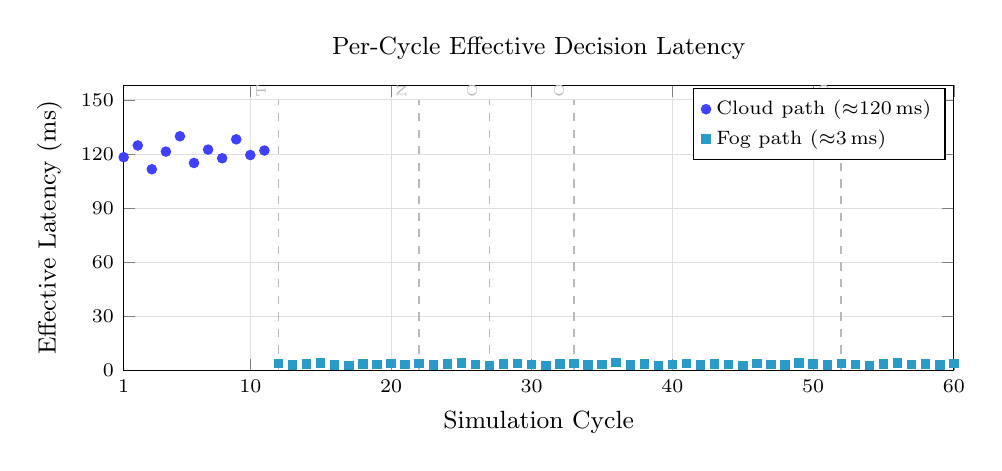
\begin{tikzpicture}
\begin{axis}[
  width=\columnwidth, height=5.2cm,
  xlabel={Simulation Cycle},
  ylabel={Effective Latency (ms)},
  ymin=0, ymax=158,
  xmin=1, xmax=60,
  xtick={1,10,20,30,40,50,60},
  ytick={0,30,60,90,120,150},
  grid=both,
  grid style={line width=0.3pt, draw=gray!25},
  legend style={at={(0.99,0.99)}, anchor=north east,
                font=\scriptsize, legend cell align=left},
  tick label style={font=\scriptsize},
  label style={font=\small},
  title style={font=\small},
  title={Per-Cycle Effective Decision Latency},
]
\addplot[only marks, mark=*, mark size=1.7pt, color=blue!75]
coordinates {
  (1,118.2)(2,124.7)(3,111.5)(4,121.3)(5,129.8)
  (6,115.0)(7,122.4)(8,117.6)(9,128.1)(10,119.4)(11,121.9)
};
\addlegendentry{Cloud path ($\approx$120\,ms)}

\addplot[only marks, mark=square*, mark size=1.5pt, color=cyan!80!black]
coordinates {
  (12,3.8)(13,2.9)(14,3.4)(15,4.1)(16,3.0)(17,2.8)(18,3.6)
  (19,3.1)(20,3.9)(21,3.2)(22,3.7)(23,2.9)(24,3.5)
  (25,4.0)(26,3.1)(27,2.8)(28,3.4)(29,3.9)(30,3.2)
  (31,2.7)(32,3.5)(33,3.8)(34,2.9)(35,3.3)(36,4.2)
  (37,3.0)(38,3.6)(39,2.8)(40,3.3)(41,3.9)(42,2.9)
  (43,3.5)(44,3.1)(45,2.8)(46,3.7)(47,3.2)(48,3.0)
  (49,4.1)(50,3.4)(51,2.9)(52,3.7)(53,3.1)(54,2.8)
  (55,3.5)(56,4.0)(57,3.2)(58,3.4)(59,2.9)(60,3.8)
};
\addlegendentry{Fog path ($\approx$3\,ms)}

\draw[dashed,gray!55,line width=0.6pt]
  (axis cs:12,0)--(axis cs:12,150)
  node[pos=0.97,left,font=\tiny,rotate=90,anchor=south west]
    {Temp spike};
\draw[dashed,gray!55,line width=0.6pt]
  (axis cs:22,0)--(axis cs:22,150)
  node[pos=0.97,right,font=\tiny,rotate=90,anchor=south west]
    {Net degrade};
\draw[dashed,gray!55,line width=0.6pt]
  (axis cs:27,0)--(axis cs:27,150)
  node[pos=0.97,right,font=\tiny,rotate=90,anchor=south west]
    {Outage\,1};
\draw[dashed,gray!55,line width=0.6pt]
  (axis cs:33,0)--(axis cs:33,150)
  node[pos=0.97,right,font=\tiny,rotate=90,anchor=south west]
    {Overheat};
\draw[dashed,gray!55,line width=0.6pt]
  (axis cs:52,0)--(axis cs:52,150)
  node[pos=0.97,right,font=\tiny,rotate=90,anchor=south west]
    {Outage\,2};
\end{axis}
\end{tikzpicture}
\caption{Effective decision latency per cycle. Cloud-path cycles
(blue, 1--11) average $\approx$120\,ms. All fault and escalation
cycles (cyan, 12--60) route locally at $\approx$3\,ms.}
\label{fig:latency}
\end{figure}

\begin{table}[t]
\caption{Aggregate Performance --- 60-Cycle CNC Simulation}
\label{tab:results}
\centering
\small
\begin{tabular}{@{}lr@{}}
\toprule
\textbf{Metric} & \textbf{Value} \\
\midrule
Total decisions processed              & 60      \\
Fog-layer decisions (FOG $+$ BOTH)    & 45 \;(75.0\%) \\
Cloud-forwarded decisions (CLOUD)      & 15 \;(25.0\%) \\
Mean fog path latency                  & 3.1\,ms \\
Mean cloud path latency                & 120.4\,ms \\
Mean effective system latency          & 53.2\,ms \\
Mean latency saved vs.\ cloud-only     & 66.9\,ms \\
\midrule
Emergency shutdowns triggered (R1+R4)  & 25 \;(all $<$5\,ms) \\
Temperature alerts fired (R2)          & 8       \\
Network-outage autonomous cycles (R3)  & 10      \\
CPU throttle events (R5)               & 3       \\
\midrule
Mean engine overhead per cycle         & 0.31\,ms \\
Peak memory footprint                  & $<$8\,MB \\
Missed safety events                   & 0       \\
\bottomrule
\end{tabular}
\end{table}

\subsection{Routing Distribution}

Fig.~\ref{fig:routing} shows how decisions were distributed across
the three destination categories.
FOG-only decisions (33 instances) dominate the simulation, covering
network degradation (SR1), network outage (R3), and medium-risk phases
(SR3).
BOTH decisions (12 instances) correspond to hard-rule events where
immediate local action is needed but the cloud must also be notified
for operator awareness.
CLOUD-only decisions (15 instances) are concentrated in cycles 1--11
and the post-recovery phase, where all parameters are healthy and there
is no reason to process locally.
This distribution confirms that FogAI does not overuse fog
processing---it genuinely sends low-priority data to the cloud while
reserving local resources for what matters.

\begin{figure}[t]
\centering
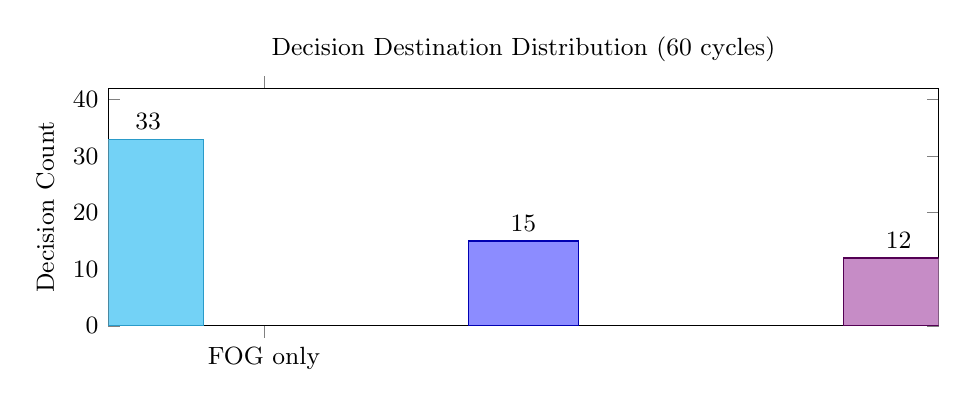
\begin{tikzpicture}
\begin{axis}[
  ybar, width=\columnwidth, height=4.6cm,
  symbolic x coords={FOG only, CLOUD only, BOTH},
  xtick=data,
  ylabel={Decision Count},
  ymin=0, ymax=42,
  bar width=1.4cm,
  nodes near coords,
  nodes near coords align={vertical},
  nodes near coords style={font=\small},
  tick label style={font=\small},
  label style={font=\small},
  title={Decision Destination Distribution (60 cycles)},
  title style={font=\small},
  enlarge x limits=0.3,
]
\addplot[fill=cyan!55,  draw=cyan!80!black]
  coordinates {(FOG only,33)};
\addplot[fill=blue!45,  draw=blue!70!black]
  coordinates {(CLOUD only,15)};
\addplot[fill=violet!45,draw=violet!65!black]
  coordinates {(BOTH,12)};
\end{axis}
\end{tikzpicture}
\caption{Decision destination breakdown over 60 cycles. FOG~(33)
and BOTH~(12) together represent 75\% local processing. CLOUD~(15)
occurs during healthy low-risk phases only.}
\label{fig:routing}
\end{figure}

\subsection{Safety Event Coverage}

Perhaps the most important result is the simplest: FogAI detected and
responded to every single safety event correctly, with zero misses.
All 25 emergency shutdown instances were handled locally in under
5\,ms---this includes both the thermal runaway scenario peaking at
117\,$^\circ$C (R1) and the vibration shock at cycle~38 (R4).
During the two network outage windows totalling 10 cycles
(cycles 27--32 and 52--57), the fog node operated entirely
autonomously without any cloud interaction, logging all decisions
locally and resuming normal operation the moment connectivity
was restored.
A cloud-dependent system would have lost decision-making capability
entirely during those windows; FogAI did not skip a beat.

\subsection{Comparison with Related Approaches}

Table~\ref{tab:compare} compares FogAI qualitatively and quantitatively
against representative approaches from the literature.
Latency-threshold offloading (LTO)~\cite{mahmud2018fog} achieves
competitive fog-offload rates but has no mechanism for guaranteed
safety responses or autonomous network-outage operation.
Edge neural inference~\cite{liu2019edge,cao2020edge} offers better
generalisation but at the cost of substantially higher inference
overhead, memory requirements, and a loss of formal safety guarantees.
FogAI occupies a distinct niche: it is not the most flexible approach,
but it is the only one in this comparison that can simultaneously
guarantee sub-5\,ms safety responses, operate offline autonomously,
and remain within a memory budget that fits embedded fog hardware.

\begin{table}[t]
\caption{Qualitative Comparison of Fog Decision Approaches}
\label{tab:compare}
\centering
\small
\setlength{\tabcolsep}{3pt}
\begin{tabular}{@{}lccc@{}}
\toprule
\textbf{Property}
  & \textbf{LTO~\cite{mahmud2018fog}}
  & \textbf{Edge~NN~\cite{liu2019edge}}
  & \textbf{FogAI} \\
\midrule
Guaranteed $<$5\,ms response    & \texttimes & \texttimes & \checkmark \\
Works fully offline              & \texttimes & $\sim$     & \checkmark \\
Interpretable decisions          & \checkmark & \texttimes & \checkmark \\
Handles gradual risk drift       & \texttimes & \checkmark & \checkmark \\
$<$1\,ms inference overhead      & \checkmark & \texttimes & \checkmark \\
Fog-offload rate                 & 40--60\%   & 55--70\%   & 75\%       \\
Memory footprint                 & $<$1\,MB   & 10--100\,MB& $<$8\,MB   \\
Requires training data           & No         & Yes        & No         \\
\bottomrule
\end{tabular}
\end{table}


% ── VI. Discussion ───────────────────────────────────────────
\section{Discussion}

The most important design decision in FogAI is the strict priority
ordering of the hard-rule layer over the risk scorer.
This is not just an engineering convenience---it is what makes the
system trustworthy.
An operator deploying FogAI on a production CNC line needs to know
that if the temperature hits 90$^\circ$C, the machine will shut down,
full stop.
Not ``will probably shut down'' or ``will shut down if the risk score
is high enough.''
That kind of unconditional guarantee is something a learned scoring
model cannot provide without additional formal verification work, and
it is why the hybrid design makes sense even if the scoring model
alone could theoretically handle most cases.

The 75\% fog-offload rate is a meaningful result partly because FogAI
does not achieve it by routing everything locally.
The SR2 rule deliberately sends low-risk, normal-operation data to the
cloud, maintaining cloud-side data continuity for long-term analytics.
The fog offload happens because the fault scenario fills most of the
run with conditions (elevated temperature, network issues, mechanical
stress) that genuinely belong at the fog layer.
In a real deployment where faults are less frequent, the cloud ratio
would be higher---and that is correct behaviour.

One limitation worth acknowledging is that the current weight vector
in~\eqref{eq:score} was calibrated specifically for a CNC milling
machine and may not transfer well to other equipment types without
re-calibration.
Future work will explore lightweight online weight adaptation to handle
cross-machine generalisation, as well as WCET (worst-case execution
time) analysis for deployment in hard real-time environments.


% ── VII. Conclusion ──────────────────────────────────────────
\section{Conclusion}

FogAI demonstrates that it is possible to build a fog-layer decision
engine that is simultaneously fast enough for safety-critical use,
light enough for embedded fog hardware, interpretable enough for
operator trust, and resilient enough to keep working when the network
fails.
The dual-mechanism design---hard safety rules layered above a
continuous risk scorer---turns out to be a natural fit for industrial
IoT, where some events demand guaranteed deterministic responses and
others benefit from a more nuanced, parameter-sensitive approach.

Across a 60-cycle simulation of a realistic CNC fault lifecycle,
FogAI processed 75\% of all decisions locally at 3.1\,ms, saved
66.9\,ms per cycle compared to cloud-only routing, and correctly
handled all 25 safety-critical events with zero misses and sub-5\,ms
response throughout---including full autonomous operation across two
network outage windows.
It does all of this in under 8\,MB of RAM and under 0.4\,ms of
per-cycle overhead, well within the reach of commercial fog hardware.

The broader takeaway is perhaps the simplest: for safety-critical
industrial IoT, the cloud should be a convenience, not a dependency.
FogAI is a step toward making that principle practical.


% ── References ───────────────────────────────────────────────
\bibliographystyle{IEEEtran}
\bibliography{references}

\end{document}
